\documentclass[11pt]{IEEEtran}

\usepackage{tikz}
\usepackage{graphicx}
\usepackage{amssymb,amsmath,amsfonts,amsthm}

\newtheorem{theorem}{Theorem}
\newtheorem{lemma}[theorem]{Lemma}
\newtheorem{proposition}[theorem]{Proposition}
\newtheorem{corollary}[theorem]{Corollary}

\theoremstyle{definition}
\newtheorem{definition}{Definition}
\newtheorem{example}{Example}
\newtheorem{observation}{Observation}


\begin{document}

\title{On Distributed Optimization in Wireless Networks: Utility Definition and Information Sharing}

\author{
%\authorblockN{David T.-H. Kao and Gareth B. Middleton}
%\authorblockA{Rice University}

David T.-H. Kao and Gareth B. Middleton\\
Rice University
%\texttt{Email: \{davidkao,gbmidd\}@rice.edu}
}

\maketitle

\begin{abstract}
In this project we examine general concepts of distributed optimization in wireless networks. After relating such optimizations to noncooperative game theory, we discuss a number of considerations regarding the design process of utility functions and how factors may impact the implementation of practical protocols. We then study the relationship between the method of information sharing in a distributed network and two commonly used classes of distributed optimization techniques. Through simulation we show that, with respect to rate of convergence, the optimization method must be tuned to the information sharing method. From this we draw a number of conclusions about necessity for joint design of game utility, information sharing and optimization methods for a distributed network.

\end{abstract}

% ---------- Section ---------- %
\section{Introduction}
When studying the performance of a wireless network, researchers should make an effort to consider not only fundamental physical constraints (such as wireless propagation), but also the personal behavior of the users themselves. To that end, a synergy between wireless networking and game theory has been developing over the past several years\cite{LTHCC07,FB04,CLD06}.  Game theory offers a wide variety of tools for use in the analysis of human behavior, which apply well to the study of networking performance.

Much of this synergy has been driven by networking researchers themselves, who begin first with a network model around which they proceed to define the game-theoretic parameters.  While this approach is not invalid, an alternative exists: to begin with the tools of game theory, and then craft and apply network model accordingly.

In this paper, we will take this second approach.  We begin with a review of concepts from distributed optimization, and then apply those to a classical wireless networking situation. First, in our review of behavior modeling, we will recognize the need for a utility function which accurately reflects the mobile wireless environment, and we will introduce an example which captures several fundamental notions therein. Second, we will study certain characteristics of utility functions that affect the practical implementation of an algorithm. Third, we examine the ways in which these utility functions are updated, and we will recognize that some amount of information sharing is required in order for the network to optimize itself. We introduce two methods of information sharing, and compare their performance.

Last, we will investigate the performance of two different optimization techniques, against the context of our previous contributions.  Our
simulation results will lead us to the final conclusion that all of these issues--utility definition, information sharing technique, and optimization method--should be jointly designed.  Ultimately, this is to say that the two approaches of combining distributed optimization and networking should be used \emph{together}, i.e. one should not ``apply'' game theory to networking or vice versa.  Rather, our paper will show that a unified approach must be taken in order to design a networking reflecting real human behavior, capable of optimizing itself in a distributed manner.

What remains of this paper is organized as follows: Section II will present preliminaries on distributed optimization, and Section III will follow with a literature review.  Sections IV - VI describe utility functions, information sharing techniques, and optimization methods, and Section VII presents our simulation results.  We conclude with discussion in Section VIII.

% ---------- Section ---------- %
\section{Preliminaries}

In this section, we briefly present basic concepts from distributed optimization and game theory which will be required to interpret the following work. For more in depth study into these two fields, the references \cite{BoydVan_book,OsborneRubinstein_book} may prove beneficial.

\subsection{Optimization Theory}
Constrained optimization problems are typically presented in the form
\begin{align}
	\text{maximize } &J(\mathbf{p})\nonumber\\
	\text{subject to } &f_i(\mathbf{p})\leq0, & i=1,\ldots,m\nonumber\\
		&g_i(\mathbf{p})=0, & i=1,\ldots,n,\nonumber
\end{align}
where $J(\cdot)$ is the objective function and $g_i(\cdot)$ and $f_i(\cdot)$ respresent sets of equality and inequality constraints. The optimization is performed over a space with a given dimension, and by considering the dual problem (optimization of the Lagrange multipliers, or ``costs'' as they are often called in the networking field) a solution can be found under certain conditions. Generally, optimization problems considered in the networking field are convex or can be mapped to convex problems, which is a sufficient condition for existence and sometimes uniqueness.

In certain situations, it is also possible to decompose the problem into a {\em separable} one by defining the original optimization as a series of optimizations over spaces of reduced dimension. An objective function is called separable if it is the sum of functions of orthogonal subspaces of the optimization space. For instance, the problem
\begin{equation}
	\max_{\mathbf{p}} \sum_{l=1}^{N} p_l^2
\end{equation}
where $\mathbf{p} \in \mathbb{R}^N$, can be separated into $N$ optimization problems.

\subsection{Relation to Game Theory}
Separable optimizations are very closely related to non cooperative game theory. In some sense, the series of $N$ separated optimizations can be viewed as a game played by $N$ individuals each seeking to maximize an individual definition of {\em utility}. In these cases, the Nash Equilibrium (the dominant solution concept in game theory) represents the solution to a separable optimization for well-behaved objective functions. 

However, the reverse mapping is not always possible. In a noncooperative game, we are not necessarily able to ``unseparate'' or consolidate the individual utilities into a single expression. Thus, by considering the framework of noncooperative game theory, we can consider the class of separable optimizations as a subset of an overall more general class of problems. 

A noncooperative {\em Game} in normal form consists of three ingredients:
\begin{itemize}
	\item A set of {\em players}
	\item For each player, a set of feasible actions or {\em strategies} 
	\item For each player, a {\em utility function} that is a function of the collection of strategies played by all players.
\end{itemize}

For the remainder of this paper we use $l \in C$ as the index of a given player (where $C = \{1,\ldots,N\}$). We also use $p_l$ to represent a strategy of Player $l$, and $p_{-l}$ to represent the strategy profile of all players besides $l$. Finally we denote the utility of Player $l$ as $u_l$. As an example of a game's relation to a distributed optimization in a wireless network, the set of players may represent a set of nodes, the strategies may represent persistence probability or power control, and utility may represent rate.

A Nash Equilibrium then is a strategy profile where no player may increase its utility by deviating from its equilibrium strategy, i.e.
\begin{eqnarray}
	\lefteqn{u_l(p_l^\star,p_{-l}^\star) \geq u_l(p_l,p_{-l}^\star)}\nonumber \\
	& & \forall p_i\in[p_l^{MIN},p_l^{MAX}], \ l \in C.
\end{eqnarray}
From an engineering viewpoint, a Nash Equilibrium has a number of desirable characteristics that describe the steady state of a distributed system.

Convergence of a particular dynamic, or way to play the game, is largely dependent on the game at hand. However, we confine our study to utility functions that are of the class $C_1$ (i.e. continuous and differentiable) and quasi-convex. This will ensure convergence of the two most common dynamics: best-reply and gradient play.

As a final note, we would like to emphasize caution with regard the the term ``utility''. This term seems to have different meanings between communites and as such, we need to differentiate between the usual networking literature usage and the game theoretic usage. Therefore, unless otherwise specified when using the term utility, we mean the function that governs the actions and reactions of users to the environment.


\section{Relation to Prior Work}
\subsection{Prior Work}
Distributed optimization and game theoretic formulations are common in wireless networks, and have been applied to medium access, congestion control, resource allocation and similar problems. Possibly the most developed study is the separability of a certain class of network utility maximization problems \cite{FB04,CLD05,NKGB00,WK03}. In some cases the optimization itself has been recast in a game theoretic framework \cite{FB04} thus justifying our approach. Though the objectives and optimization spaces of these results vary, the common theme is that under the network utility maximization framework, the Lagrange multipliers (costs) can be used to direct a separable optimization process. In the case of wireless networks however, the prices cannot be dictated by a physical link and must originate organically from the interaction of devices. Consequently, the price specification process may be wrought with error and delay or the network must accomodate overhead to exchange information. 

At the other end of the spectrum, there have been a number of significant contributions in modelling networks as purely noncooperative in nature. For example, medium access control is particularly well suited for game theoretic analysis since the contention is inherently noncooperative. In \cite{CLD06} random access protocols were cast in this framework, and the reverse-engineering of 802.11 Exponential Backoff mechnism as a noncooperative game was presented recently in \cite{LTHCC07}. The authors defined, based on specifications in the standard, the utility function of a wireless users utilizing exponential backoff.

\subsection{Our Contributions}
In the work discussed above, two key issues present themselves as gross factors in determining the network solution and optimization method:

\begin{itemize}
  \item Utility function definitions
  \item Information sharing techniques
\end{itemize}

Prior work has assumed, conveniently, either utility functions with properties that simplify analysis (ie, concavity) or ones
based on existing protocols that are unfortunately opaque. In this work, we set out to fully describe how utility functions may be designed in general. We also present formalized descriptions of two major design characteristics that affect the method and outcome of the distributed optimization. We use as examples well known network optimization problems and discuss briefly how their utility definitions relate to practical considerations in system design.

After studying these utility functions, we will look further at the requirements for a distributed optimization; namely, how the nature of the information required for the optimization is passed around the network. We show that the nature of the information sharing method greatly affects which distributed optimization technique is best. 





%-----------------------------------------------------------
\section{Design of Utility Functions}
\subsection{Environment-Driven Utility Functions}
The solution to an optimization problem, as well as the algorithm to find such a solution, will depend heavily on the selection of the utility function over which the optimization is performed. We first present the general process for designing a utility function for a particular problem based on the system constraints and objective.
%
In the following subsections, we discuss two considerations regarding utility functions. It is intended that these considerations may provide an engineer with a partial recipe for the design of a distributed wireless network. For each, we provide examples to help illustrate the implications on practical considerations. 
%
To simplify the explanation, in each example the subspace over which each user's individual optimization occurs is its persistence probability, defined here:
\begin{definition}[Persistence Probability]
	A user's \emph{persistence probability} ($p_l$), indexed by $l$, is their probability of attempting data transmission, when given the opportunity (e.g. in the case of 802.11, during backoff, in the case of slotted ALOHA, in any slot).
\end{definition}

Here, we present a simple example of the process one would take in order to define a utility function for a given scenario.

\begin{example}[``Smiles-per-Watt'']
Consider a single-clique network of $n$ users in an unlicensed band. Let's assume that these users are
\begin{itemize}
	\item Selfish
	\item Interested in maximizing their quality of service (QoS)
	\item Concerned with energy consumption 
\end{itemize}
In other words each user has a particular demand for bandwidth but its usage of the medium is tempered by an unwillingness to spend too much energy on a transmission. Furthermore, each user completely disregards others in the network.\footnote{This may model, for instance, independently designed low power devices like Bluetooth}

We first specify the function which represents the user's QoS.  With respect to throughput, let the following QoS function for User~$l$ be given:
\begin{equation}
  Q_l(s) \triangleq M \left(\frac{\tanh\left[As-s_0\right] - \tanh\left[-s_0\right]}{1-\tanh\left[-s_0\right]}\right).
  \label{eq:qos1}
\end{equation}
where the constants $M, A, s_0 > 0$ are scaling and shifting values affecting the shape of the curve, which can be adapted to the service being considered. Of these, the parameter $A$ conveys the most about User~$l$'s throughput demand. As $A$ increases, the $Q_l$ is compressed and User $l$ becomes satisfied at a lower rate. We have plotted an example of the QoS function in Figure \ref{fig:QoS}.

This QoS function is of some rate $s$, but is not yet related to persistence probability $p_l$.  We can write this relation as
\begin{equation}
  s = L p_l \prod_{j \in C\setminus l} (1-p_j)
  \label{eq:thru}
\end{equation}
where $L$ denotes packet length and $C$ is the set of indices of users in the clique. By substitution of (\ref{eq:thru}) we arrive at the QoS as a function of the persistence probability $p_l$.

\begin{eqnarray}
  \lefteqn{Q_l(p_l) \triangleq}\nonumber\\
  & M \left(\frac{\tanh\left[A\left(L p_l \prod_{j \in C\setminus l} (1-p_j)\right)-s_0\right] - \tanh\left[-s_0\right]}{1-\tanh\left[-s_0\right]}\right)
\end{eqnarray}

We now scale the user satisfaction by a penalty term reflecting energy use. Thus we arrive at our utility function:
\begin{equation}
  u_l(p_l) \triangleq \frac{Q_l(p_l)}{kp_l},
  \label{eq:util}
\end{equation}
where $k$ represents a scaling constant on battery drain.  The units of $u_l$ can be thought of as energy efficient satisfaction or ``smiles per watt.'' A plot demonstrating typical characteristics of $u_l(p_l)$ appears in Figure~\ref{fig:QoS}.


%\usepackage{graphics} is needed for \includegraphics
\begin{figure}[htp]
\begin{center}
\begin{tikzpicture}[domain=0:1, xscale=6, yscale=3, samples=50]
\draw[help lines,xstep=0.2,ystep=.5 ] (0,0) grid (1,1.5);
\draw[-latex] (-0.03,0) -- (1.03,0) node[right] {$p$};
\draw[-latex] (0,-.05) -- (0,1.65) node[above] {};
 
 \foreach \t in {.2,.4,.6,.8,1}{\draw (\t,.01) -- (\t,-.01) node[below] {$\t$};}
 \draw[red, smooth, thick] plot file{points/document.qos.table} node [right,
 below] {$Q(p)$}; 
 \draw[blue, smooth, thick] plot file{points/document.u.table}
 node [right,above] {$u(p)$};

%\draw[color=red]plot[id=qos]function{(tanh(5*(x-.5))-tanh(5*(0-.5)))/(1-tanh(5*(0-.5)))};
%\draw[color=blue]plot[id=u]function{(tanh(5*(x-.5))-tanh(5*(0-.5)))/(x*(1-tanh(5*(0-.5))))};
\end{tikzpicture}
\caption{Quality of Service and Utility for our function.}
\label{fig:QoS}
\end{center}
\end{figure}
\end{example}

In this particular example, the design was straight forward and unhampered by overhead or global optimization considerations.
Realistically however, these are two of the most prominent considerations in the design of wireless networks.

\subsection{Aggregation of Utility Parameters}
A common concern from a design standpoint is the overhead associated with a protocol. We intend to quantify this concept with an index defined by the dimensionality of the parameter(s) used in each individual utility definition, relative to dimensionality of possible network states. For example, if the information from the network needed by a user for distributed optimization can be expressed as a single-dimensional parameter, the necessary overhead for conveying control information can be significantly reduced or eliminated altogether. On the other hand, if the dimensionality of information grows with the size of the network (e.g. the unique identities of users is relevant to a utility definition), all of that information must be shared. 

Clearly, this has implications towards the method of information sharing, and implicitly scalability of the network. We now formally define an index describing the aggregation of parameters that are components of utility.
\begin{definition}[Information Growth Factor]
	Consider a single-clique network of $n$ users involved in a distributed optimization. Let $I_l$ be the information vector of the $l^{th}$ link and $| I_l |_n$ be the minimum number of bits needed to represent $I_l$ in the $n$ user network. The information growth factor (IGF), $G$, is defined in terms of the amount of necessary information needed by any single user to perform its individual optimization by the following relation.
	\begin{equation}
		\max_l |I_l|_n = \mathcal{O}(n^G) 
	\end{equation}
\end{definition}

We now present an example where we compute this factor. 
\begin{example}[Exponential Backoff Game \cite{LTHCC07}] 
Consider the game described in \cite{LTHCC07}. Here the utility of a User~$l$ was defined as \footnote{The original utility was defined in more general terms however here we assume binary exponential backoff for clarity.}
\begin{align}
	u_l(p_l,p_{-l}) &=& p_l^2\left(\frac{1}{4} - \frac{1}{3}p_l\right)\prod_{j \in C\setminus l}(1-p_j)\nonumber \\
	& & -\frac{1}{6}p_l^2\left(1 - \prod_{j \in C\setminus i}(1-p_j)\right).
	\label{eq:rem}
\end{align}

Notice that the expression
\begin{equation}
	\prod_{j \in C\setminus l}(1-p_j)
\end{equation}
exists independent of any persistence probability selection on the part of User~$l$.

Thus for the exponential backoff game, the parameter describing the network to User~$l$ is independent of network size. As a result the dimensionality of this parameter is one and $G = 0$.
\end{example}

The impact the IGF has on overhead can be best seen by considering the situation described by the exponential backoff game. The exponential backoff mechanism in the 802.11 standard requires next to no overhead; the reception of an ACK (or lack thereof) is in fact the only feedback received from the system. Furthermore, as more nodes join such a network, the method in which our original user receives information regarding the state of network devices remains the same: {\em no additional overhead is needed as the network grows}. 

Clearly then, a low IGF leads to cases amenable to large networks, whereas a high IGF suggests that optimization comes at a significant cost in overhead. Finally, one might interpret this from a design point of view as a method of reducing overhead at the cost of true system optimality. If a particularly information hungry definition of utility is altered slightly, then one may be able to trade off optimality for reduction in overhead which may in turn lead to overall improvement in system performance.



\subsection{Implicit Cooperation in Noncooperative Games}
In a large body of work \cite{FB04,CLD05,NKGB00,WK03}, global optimizations have been recast as separable distributed optimizations. However, in noncooperative games utility functions are generally defined in a selfish manner. Here an explanation is given for true collaborative optimization in a distributed network. We explain the mechanism behind this collaboration in game theoretic terms and discuss how this may be used to design global optimizations that can be decomposed to distributed algorithms. On another note, this formulation may also be used to reverse-engineer a number of distributed or noncooperative protocols, and to describe the underlying collaborative optimizations.

The concept of a potential game is well known in game theoretic literature:
\begin{definition}[Potential Game]
	A game is said to be a \emph{potential game} if there exists a global function, the potential function $U(\mathbf{p})$, such that if any single user increases/decreases its utility by adjusting its strategy, the potential function increases/decreases as well, i.e.
	\begin{align}
		u_l(p_l,p_{-l}) \geq u_l(p_l',p_{-l}) &\Longrightarrow \nonumber \\
			&U(p_l,p_{-l}) \geq U(p_l',p_{-l})
	\end{align}
\end{definition}

Thus, if a game has a global function which can be extremized by adjusting individual user parameters, then the users are essentially ``cooperating,'' even if their utility functions are strictly selfish. Thus we say that the cooperation is {\em implied} or embedded in the individual selfish utility definitions. Furthermore, if the global function satisfies convexity/concavity constraints, the solution will be unique for the network. Consider the following well known network optimization problem.

\begin{example}[Network Utility Maximization]
	Let us consider the general problem of network utility maximization \cite{FB04,LCC07,CLD05,NKGB00,WK03}. We can easily claim two things.
	\begin{enumerate}
		\item The network utility expression can be used to define both the {\em selfish game}
				\footnote{Again notice that the game utilities are not necessarily the individual summed components in the global network utility definition. The game utilities describe the actions of each user with respect to the actions of others, whereas in the network utility definition, utility is an abstract concept utilized in describing some global objective.} 
			 utilities for {\em all} users.
		\item As a result, the network utility expression also defines a potential function for the distributed optimization.
	\end{enumerate}
	As noted by the authors, concavity of the network utility relative to any single user's actions permit this global maximization in a distributed framework.
\end{example}

As a result, if it is desired for a network to maximize some global function in a distributed and separable manner, then the function itself must be consistent with the definiton of a potential function. If the desired function does not satisfy this constraint, then it may be necessary to tweak the definition in order to produce a separable problem. This is, in fact, a common approach as some situations \cite{CLD05} have necessitated a relaxation or perturbation of the original objective in order to produce a problem capable of being solved in a distributed manner.


% ---------- Section ---------- %
\section{Information Sharing Methods}

In the previous section, we discussed the implications of utility functions and the parameters which comprise their calculation. In much of the previous work, these parameters have been assumed known to all nodes ``free of charge,'' so that a node may compute its utility (or actions) directly. However, such information is generally not available to all nodes, and instead must be shared. In this section, we discuss some methods which allow network parameters to be shared among nodes. For this discussion, we assume each node requires knowledge of some function of the network traffic which necessitates knowledge of other users persistence probabilities. 


\subsection{Measurement Methods}

One way for a node to estimate network traffic is to measure it, by listening to packet transmissions.  From a measurement of packet transmissions, a node can then estimate other nodes' persistence probabilities.  If the utility definition permits (when IGF is zero), one can measure aggregate network traffic by simply sensing for idle periods in the medium. On the other hand if a user requires specific information regarding each other user in the network, we can allow nodes to decode packet headers to obtain specific estimates $\hat{p_l}$ of node~$l$'s persistence probability.  With all of these estimates, the node can then solve a simple system of equations.

\subsection{Message Passing}

An alternative would be for each node to include its persistence probability as a field in its packet header, which would then be decoded by all other nodes in the clique. In this way, other nodes would be perfectly informed of all information, though they are required to decode all packet headers and unlike the measurement method, no information is gathered during periods of contention (collision). Notice that the concept of a control channel seen in many protocol specifications also falls under this category of information sharing.

\section{Optimization Techniques}

After nodes have estimated or obtained network parameters, they must update
their strategies accordingly.  We now discuss some optimization (update) techniques. 

\subsection{Best-Reply}

In this case, a node computes its optimal response \emph{ceteris paribus}, assuming that the rest of the network does not change. 
 \begin{example}[Chess]
In a chess game, the best-reply strategy would be to ignore
any potential future move of the opponent and attempt an immediate checkmate. 
\end{example}

\subsection{Gradient Descent}
This method is similar to Best Reply, except that rather than implementing its optimal response, a node moves \emph{in the direction} of the optimal response, the distance towards which is governed by some weighting parameter. In systems when utility may be poorly behaved (nonconcave, non continuous, etc.) a subgradient method is typically proposed.

\begin{example}[Chess]
In a chess game, the gradient descent strategy would be to
forecast a few moves ahead, and move optimally in light of that forecast.
\end{example}

\subsection{Interaction between Information and Optimization}
Note that these techniques are quite different: Best-Reply is aggressive,
potentially making drastic changes to a node's behavior based on its network
information.  If this information is in error, Best-Reply may cause the node to
operate in a substantially sub-optimal way.  We are therefore motivated to
study the interaction between network information and the optimization
technique, to see if some techniques are better suited to certain information
estimates.  This study will be conducted using simulation, presented below.

\section{Simulation Results}
\subsection{System Configuration}

We model a fully backlogged slotted ALOHA system, in which the persistence probability for each node is exactly the probability of transmission in a given slot.  All flows are one-hop, and we assume a single clique only.  We will study a variety of information sharing techniques, though we will assume that the utility function used is the 802.11 exponential backoff-inspired function appearing in (\ref{eq:rem}).  Unless otherwise stated, we assume a two-node network with a unique solution. For the Measurement method on information sharing we analyze both aggregate and individual parameter cases, and for the Message Passing method we assume that these messages are ``piggy-backed'' on actual data transmission packets. These information sharing methods are also compared with a genie aided information sharing system employing the same optimization methods.

\subsection{Information Sharing and Optimization}

Acting on the intuition that the network's information sharing method and distributed optimization technique are related, we first explore the interaction between each optimization technique and the two information sharing methods under consideration.  To begin, we consider the measurement method of gathering information.  As shown in Figure~\ref{fig:BestReply}, the persistence probability is significantly unstable when Best Reply is fed with measured network information, and tends to oscillate wildly about the genie aided, ideal solution.

This noise in the measurement scenario  arises from the fact that measured information is subject to some error.  The error, likely different in the next measurement, causes Best Reply to choose differing persistence probabilities over time.  

% Best Reply figure
\begin{figure}[htp]
\begin{center}
  \begin{tikzpicture}[xscale=1.0, yscale=25]

  \draw[help lines,xstep=1,ystep=0.05 ] (0,0.3) grid (6,0.5);
  \draw[-latex] (0,0.3) -- (6.1,0.3);
  \draw[-latex] (0,0.3) -- (0,0.51);
  \small
   \foreach \t in {0,1,2,3,4,5,6}{
   \draw (\t,.305) -- (\t,0.295) node[below] {$\t$};
   }

  \small
   \foreach \t in {0.30,.35,0.4,0.45,0.5}{
   \draw (.1,\t) -- (-.1,\t) node[left] {$\t$};
   }

%  \draw[red, smooth, thick] plot file{document.qos.table} node [right, below]
%  {$Q(p)$};

   \draw[blue, smooth, thick] plot file{points/plot1_BR_m.table} node [right] {Meas};
   
   \draw[red, smooth, thick] plot file{points/plot1_BR_p.table}  node [above
   right] {Ideal};
     
  \node (xl) at (3, .27) {Time (sec)};
  \node (yl) at (-1, .4) [rotate=90] {$p_i$};
  \node (tl) at (3, 0.52) {Best Reply};


  \end{tikzpicture}
  \caption{Performance of the Best Reply strategy when using ideal and measured
  network information.}
  \label{fig:BestReply}
\end{center}
\end{figure}

Next, we consider the Gradient Descent method under the same conditions. Intuitively, one might guess that the more gradual nature of Gradient Descent may mitigate some of the unstable approach of Best Reply. The results, shown in Figure \ref{fig:graddesc}, seem to confirm this hypothesis.  Here, we note that the Measurement techniques performs comparably to even the genie-aided gradient descent. This is a result of Gradient Descent moving ``slowly enough'' that errors in measurement are averaged out over time.  Note that even with perfect information from the genie-aided Gradient Descent takes some length of time to converge; this length is dictated by the Gradient Descent step size. Consequently, it may be possible to tune this convergence speed by increasing the step size. However, when step size is very large, Gradient Descent degenerates to Best Reply. Therefore there seems to be some tradeoff between the rate of convergence and stability about the solution for Measurement based networks.

% Gradient Descent figure
\begin{figure}[tp]
\begin{center}
  \begin{tikzpicture}[xscale=1.0, yscale=25]

  \draw[help lines,xstep=1,ystep=0.05 ] (0,0.3) grid (6,0.5);
  \draw[-latex] (0,0.3) -- (6.1,0.3);
  \draw[-latex] (0,0.3) -- (0,0.51);
  \small
   \foreach \t in {0,1,2,3,4,5,6}{
   \draw (\t,.305) -- (\t,0.295) node[below] {$\t$};
   }

  \small
   \foreach \t in {0.30,.35,0.4,0.45,0.5}{
   \draw (.1,\t) -- (-.1,\t) node[left] {$\t$};
   }

%  \draw[red, smooth, thick] plot file{document.qos.table} node [right, below]
%  {$Q(p)$};

   \draw[blue, smooth, thick] plot file{points/plot1_GR_m.table} node
   [below right] {Meas};

   \draw[red, smooth, thick] plot file{points/plot1_GR_p.table} node [above
   right] {Ideal};

     
  \node (xl) at (3, .27) {Time (sec)};
  \node (yl) at (-1, .4) [rotate=90] {$p_i$};
  \node (tl) at (3, 0.52) {Gradient Descent};

  \end{tikzpicture}
  \caption{Performance of the gradient descent algorithm when using ideal and
  measured network information.}
  \label{fig:graddesc}
\end{center}
\end{figure}

We are next prompted to study the convergence time of our techniques across the network when information is gained through Measurement. For our purposes, we will deem the system to have \emph{converged} if all persistence probabilities are within some small $\epsilon$ of their equilibrium values.  Jittery probabilities, when shared, can cause equal jitter in the probabilities of other nodes--we conjecture that this effect becomes magnified as the size of the network increases, especially if each node is using individually specified information.  In Figure~\ref{fig:IndAggconvergence}, we plot the convergence time of the system when both individual and aggregate parameters are measured, as a function of network size.  To isolate the effects under consideration, we assume a Message Passing information sharing method.

We see that when aggregate parameters serve as inputs to utility functions, convergence time remains low regardless of network size.  Contrariwise, a larger network suffers from extremely long convergence time, when individual parameters are used in utility functions.  The intuition behind this result is that, when network parameters are aggregated, variations across users tend to cancel out, such that the aggregate parameter is stable as time evolves.  In contrast, individual utility functions may change significantly over time, causing utility updates to be similarly jittery.

% Ind-Agg convergence time
\begin{figure}[htp]
\begin{center}
    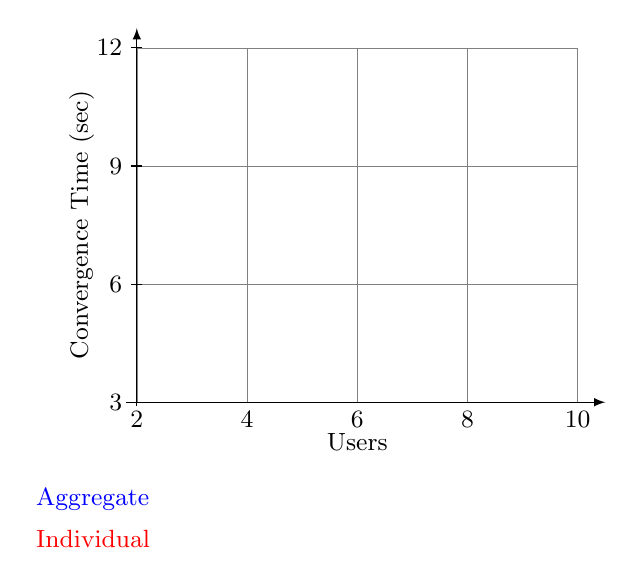
\begin{tikzpicture}[xscale=.7, yscale=.5]

  \draw[help lines,xstep=2,ystep=3 ] (2,3) grid (10,12);
  \draw[-latex] (1.8,3) -- (10.5,3);
  \draw[-latex] (2,2.9) -- (2,12.5);
  \small
   \foreach \t in {2,4,6,8,10}{
   \draw (\t,3.01) -- (\t,2.99) node[below] {$\t$};
   }

  \small
   \foreach \t in {3,6,9,12}{
   \draw (2.1,\t) -- (1.9,\t) node[left] {$\t$};
   }

%  \draw[red, smooth, thick] plot file{document.qos.table} node [right, below]
%  {$Q(p)$};

   \draw[blue, smooth, thick] plot file{points/plot2_AG.table} node [above
   right] {Aggregate}; 
   \draw[red, smooth, thick] plot file{points/plot2_IN.table} node
   [below right] {Individual};

  \node (xl) at (6, 2) {Users};
  \node (yl) at (1, 7.5) [rotate=90] {Convergence Time (sec)};

  \end{tikzpicture}
  \caption{Convergence times of the network when both global and individual
  utility functions are being optimized.  Information is assumed to be ideal,
  shared using Message Passing.}
  \label{fig:IndAggconvergence}
\end{center}
\end{figure}

We now consider convergence time when information is shared via Message-Passing under our two  classes of optimization techniques. We see from Figure~\ref{fig:convergence2} that Best Reply reaches convergence fastest for all network sizes, though Gradient Descent sees performance improvement as the number of users increases.  We have also plotted the convergence time for a network measuring an aggregate parameter using Gradient Descent; notice that this curve tracks Gradient Descent very closely. This suggests that if Message Passing is available as an option, and the overhead demands are bearable, Measurement information sharing is never a better option. 


% Convergence time
\begin{figure}[htp]
\begin{center}
  
  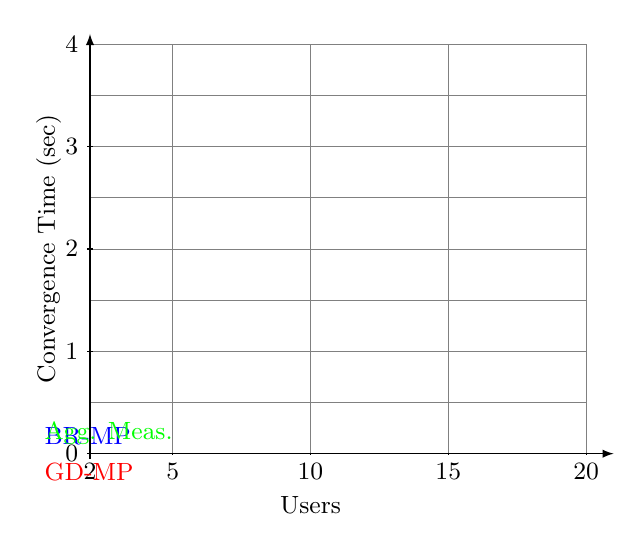
\begin{tikzpicture}[xscale=.35, yscale=1.3]

  \draw[help lines,xstep=5,ystep=.5 ] (2,0) grid (20,4);
  \draw[-latex] (1.9,0) -- (21,0);
  \draw[-latex] (2,-.05) -- (2,4.1);
  \small
   \foreach \t in {2,5,10,15,20}{
   \draw (\t,.01) -- (\t,-.01) node[below] {$\t$};
   }

  \small
   \foreach \t in {0,1,2,3,4}{
   \draw (2.1,\t) -- (1.9,\t) node[left] {$\t$};
   }

%  \draw[red, smooth, thick] plot file{document.qos.table} node [right, below]
%  {$Q(p)$};

   \draw[blue, smooth, thick] plot file{points/plot4_BR.table} node [above
   right] {BR-MP}; \draw[red, smooth, thick] plot file{points/plot4_GR.table}
   node  [below right] {GD-MP}; \draw[green, smooth, thick] plot file{points/plot4_M.table}
   node [above right] {Agg. Meas.};

  \node (xl) at (10, -0.5) {Users};
  \node (yl) at (.5, 2) [rotate=90] {Convergence Time (sec)};

  \end{tikzpicture}
  
  \caption{Convergence time when using Best Reply with message passing, gradient
  descent with message passing, and aggregate parameter optimization.}
  \label{fig:convergence2}
\end{center}
\end{figure}

Last, we consider a comparison of our optimization techniques using the ideal Message Passing scheme.  This result is shown in Figure \ref{fig:GDMP}.  Note that, as before, Gradient Descent takes significantly longer to converge than Best Reply. These simulations for our relatively simple model suggest that for well behaved definitions of utility, latency in receiving information has less of an impact than error in that information.

% GD-BR under message passing
\begin{figure}[htp]
\begin{center}
    \begin{tikzpicture}[xscale=1.0, yscale=25]

  \draw[help lines,xstep=1,ystep=0.05 ] (0,0.3) grid (6,0.5);
  \draw[-latex] (0,0.3) -- (6.1,0.3);
  \draw[-latex] (0,0.3) -- (0,0.51);
  \small
   \foreach \t in {1,2,3,4,5,6}{
   \draw (\t,.305) -- (\t,0.295) node[below] {$\t$};
   }

  \small
   \foreach \t in {0.30,.35,0.4,0.45,0.5}{
   \draw (.1,\t) -- (-.1,\t) node[left] {$\t$};
   }

%  \draw[red, smooth, thick] plot file{document.qos.table} node [right, below]
%  {$Q(p)$};

   \draw[blue, smooth, thick] plot file{points/plot3_BR00.table} node [below
   right] {BR-MP};
   \draw[blue, smooth, thick] plot file{points/plot3_BR01.table};
   
   \draw[red, smooth, thick] plot file{points/plot3_GR00.table} node [above
   right] {GD-MP};
   \draw[red, smooth, thick] plot file{points/plot3_GR01.table};  
     
  \node (xl) at (3, .27) {Time (sec)};
  \node (yl) at (-.9, .4) [rotate=90] {$p_i$};

  \end{tikzpicture}
  \caption{Performance of Gradient Descent and Best Reply when using
  message-passing.}
  \label{fig:GDMP}
\end{center}
\end{figure}


\section{Summary and Discussion}

\subsection{Summary}

In this paper, we have reviewed several issues in the design of networks using distributed optimization theory.  Our discussion of utility
functions revealed the considerations a designer should take into account when assigning functions to nodes, and presented examples of several different types of legitimate utility functions.

Two key ideas arose from this discussion: the concept of implicit cooperation, and the notion of aggregate and individual parameterization. We are able to show that, even if utility functions are defined to be purely selfish, some type of cooperation may still be implied by using a \emph{potential} optimization function. This may be of particular use in the analysis of wireless networks, since users are assumed to be naturally selfish, though some level of cooperation is required for the network to operate in a feasible manner.

The issue of aggregate and individual parameterization concerns the input parameters to the node's utility functions--how much network information they require to choose their behavior.  This led directly to our study of information sharing, in which we presented two techniques: the low-overhead, immediately implementable Measurement method and the ideal Message Passing method.

We studied these methods in the context of two different classes of update techniques at the nodes, Gradient Descent and Best Reply.  The comparison of these behaviors was conducted using simulations.

\subsection{Discussion}

The key result arising from this study is the level of interaction between utility functions, information sharing technique, and optimization method. These seemingly independent arenas of Distributed Optimization Theory turn out to be intimately related in the context of a wireless network, as our simulation results borne out: some combinations of sharing techniques worked well with certain optimization methods, others were disasterous.

A future study should take this link into account when designing these two components of the system: how to ensure low-overhead information sharing yet stable and rapid convergence to optimal solutions.  The techniques we surveyed here are not optimal, but perhaps a jointly designed information-sharing-optimization method exists.

However, this pursuit should be conducted in the context of the network at hand.  In our case, we are considering fully backlogged nodes, and so jittery or unstable persistence probabilities are detrimental to system performance. However, if the application running on the network is more bursty in nature, the network can tolerate a slower convergence time and the optimal schemes may turn out to be different.  In that vein, an \emph{adaptive} optimization and sharing scheme should be pursued.

\bibliographystyle{IEEEtran}
\bibliography{IEEEabrv,elec537proj,books}
\begin{biography}[{\includegraphics[width=1in,height=1.25in,clip,keepaspectratio]{./gbm.jpg}}]{Gareth Bruce Middleton} 
Gareth enjoyed ELEC 537 thoroughly. His favorite lecture was the presentation of Djikstra's Algorithm applied to minimum weight routing and favorite paper was Kleinrock and Tobagi's ``Packet Switching in Radio Channels: Part I - Carrier Sense Multiple-Access Modes and Their Throughput-Delay Characteristics''.
\end{biography}
\begin{biography}[{\includegraphics[width=1in,height=1.25in,clip,keepaspectratio]{./dtk.jpg}}]{David Teh-Hwa Kao} 
David found ELEC 537 very informative and enlightening. His favorite lecture was the application of Markov Processes Theory to protocol analysis and favorite paper was Bianchi's ``Performance analysis of the IEEE 802.11 distributed coordination function''.
\end{biography}
\end{document}